\documentclass[a4paper]{article}
\usepackage{ctex}
\usepackage{geometry}
\usepackage{amsmath}
\usepackage{ulem}
\usepackage{graphicx}
\usepackage{siunitx}
\usepackage{enumitem}
\usepackage{multirow}
\usepackage{adjustbox}
\usepackage[hidelinks]{hyperref}
\usepackage{listings}
\usepackage{xcolor}
\lstset{
    language=Matlab,
    basicstyle=\sffamily\footnotesize,
    keywordstyle=\color{blue},
    commentstyle=\color{gray},
    stringstyle=\color{red},
    numbers=left,
    numberstyle=\tiny\color{gray},
    stepnumber=1,
    numbersep=5pt,
    backgroundcolor=\color{white},
    showspaces=false,
    showstringspaces=false,
    showtabs=false,
    frame=single,
    tabsize=4,
    captionpos=b,
    breaklines=true,
    breakatwhitespace=false,
    escapeinside={\%*}{*)},
}

\geometry{left=2.5cm, right=2.5cm, top=2.5cm, bottom=2.5cm}
\zihao{-4}

\begin{document}

\noindent\textbf{班级：24级整合科学班} \hspace{1cm} \textbf{学号：2400017802} \hspace{1cm} \textbf{姓名：冯翊展} \hspace{1cm} \textbf{评分：}\\
\textbf{同组学生：胡家豪 \ 陈天铭 \ 侯树宽} \\
\textbf{实验名称：使用布朗运动测量玻尔兹曼常数和阿伏伽德罗常数}   \hfill \textbf{实验日期：2025年3月14日} 

\hrule
\vspace{3mm}

\begin{enumerate}[label=\chinese*.,left=0pt]
    \item 实验目的
    \\
    使用用荧光显微镜追踪并记录荧光微球的位置，计算得到微球的扩散系数，并据此计算玻尔兹曼常数和阿伏伽德罗常数。
    
    \item 实验内容
    \\
    在掌握显微镜的基本工作原理和使用方法，使用荧光显微镜观察并记录流道中荧光微球的布朗运动，并利用 ImageJ、Matlab 等软件对所得图像进行数据处理与分析，
    
    \item 基本原理
    \begin{enumerate}[label=\arabic*.,left = 0pt]
        \item 随机游走模型：考虑若干粒子在一维空间上随机的左右运动，每隔 $\tau$ 秒粒子运动 $\delta$ 的距离，左右概率相等，那么第 $i$ 个粒子在 $n$ 步之后的位置应该是：
        $$x_i(n) = x_i(n-1)\pm\delta.$$
        若共有 $N$ 个粒子，则其均方平均位置符合递推式:
        $$\langle x^2(n)\rangle = \frac{1}{N} \sum_{i=1}^N \left[ \langle x_i^2(n-1)\rangle \pm 2\delta\right \langle x_i(n-1)\rangle +\delta^2] = \langle x^2(n-1) \rangle + \delta^2.$$
        故 $\langle x^2(n) \rangle = n\delta^2$。令 $t=n\tau$, 并引入扩散系数 $D = \delta^2 / 2\tau$，即得
        $$\langle x^2(t)\rangle = 2Dt.$$
        对于二维游走，由于每个维度分别符合一维随机游走模型，因此
        $$\langle r^2(t) \rangle = 4Dt.$$

        \item Stokes-Einstein 关系：在雷诺数较低的情况下，光滑球形刚体在流体中所受阻力满足Stokes公式：
        $$f = \gamma v, \quad \gamma=6\pi\eta r.$$
        对于物体在流体中的随机游走过程，有 Einstein 关系式：
        $$D= \frac{kT}{\gamma}.$$
        联立得到：
        $$D = \frac{kT}{6\pi\eta r}.$$

        \item 布朗运动的高斯分布：考虑粒子从原点出发，经历 $n$ 步后位于 $x$ 的概率是
        $$P(x) = \binom{n}{\frac{n}{2}+\frac{x}{2\delta}} =\frac{n!}{\left(\frac{n}{2}+\frac{x}{2\delta}\right)! \left( \frac{n}{2}-\frac{x}{2\delta}\right)!}.$$
        $n$ 较大时，使用斯特林近似，
        \begin{align*}
            \ln{P(x)} & \approx n\ln n - \left(\frac{n}{2}+\frac{x}{2\delta}\right) \ln{\left(\frac{n}{2}+\frac{x}{2\delta}\right)}- \left(\frac{n}{2}-\frac{x}{2\delta}\right) \ln{\left(\frac{n}{2}-\frac{x}{2\delta}\right)} \\
            & = -\frac{n}{2}\ln{\left(1-\frac{x^2}{n^2\delta^2}\right)}+\frac{x}{2\delta}\ln \left(1-\frac{2x}{n\delta+x}\right)+n\ln 2 \\
            & \approx \frac{x^2}{2n\delta^2}-\frac{x^2}{n\delta^2}+n\ln 2 \\
            & = -\frac{x^2}{2n\delta^2}+n\ln2 
        \end{align*}
        故 $P(x) \propto \exp{\left(-\frac{x^2}{2n\delta^2}\right)}=\exp{\left(-\frac{x^2}{4Dt}\right)}$，即符合高斯分布。进一步归一化得到
        $$P(x) = \frac{1}{(4\pi Dt)^{1/2}}e^{-\frac{x^2}{4Dt}}.$$
        对于二维布朗运动，由于粒子在两个方向上的运动独立，故
        $$P(x,y) = P(x) \cdot P(y) = \frac{1}{4\pi D t} e^{-\frac{x^2+y^2}{4Dt}} = \frac{1}{4\pi Dt} e^{-\frac{r^2}{4Dt}}$$

        \item 玻尔兹曼常数和阿伏伽德罗常数：由理想气体方程立即得到
        $$PV=nRT = kN_\text{A}T \implies N_\text{A} =\frac{R}{k}.$$
    \end{enumerate}
    
    \item 仪器与试剂
    \begin{enumerate}[label=\arabic*.,left = 0pt]
        \item 仪器：荧光显微镜，相机，$\qty{100}{\micro \litre}$/$\qty{1000}{\micro \litre}$移液枪，载玻片，盖玻片，离心管，镊子，胶条
        \item 试剂：$\qty{100}{\micro \litre}$荧光微球母液，蒸馏水，指甲油
    \end{enumerate}

    \item 实验步骤
    \begin{enumerate}[label=\arabic*.,left = 0pt]
        \item 取洁净载玻片，沿矩形长边缘黏合适当长条形胶条，平稳盖放盖玻片，使得胶条在盖玻片与载玻片间形成可让微球自由运动的罅隙。
        \item 取 \qty{10}{\micro \litre} 的荧光微球母液，利用微量可调移液器依次稀释至 $\times100$、$\times1000$、$\times10000$ 倍数。
        \item 沿流道边缘缓慢滴加特定稀释倍数的微球悬液，使悬液均匀渗透进流道的罅隙且不在盖玻片下方残留气泡， 用指甲油封装盖玻片四周。 调整荧光显微镜使其投射蓝光，在 $\times100$ 物镜下预观察。若视野范围内微球密度适当（便于单个微球追踪） ， 则切换至显微镜相机观察。 若视野范围内微球过密或过疏， 则重新选定微球悬液的稀释倍数， 并重复上述仪器调整的操作直至密度恰当。
        \item 相机记录：选取特定视野并固定，用相机在 \qty{40}{\second} 内持续记录视野内微球的二维布朗运动。 若记录过程中微球脱焦， 可略微调整细准焦螺旋使小球重新对焦。 重复上述记录操作直到成功获得 $10$ 次微球二维布朗运动的视频记录。若在实验操作过程中出现视野范围内微球沉降（即视野内微球几乎无水平方向上运动）的情况，在及时更换流道后再进行后续的数据记录。
        \item 实验结束后，保存视频数据，清洁显微镜物镜和载物台，整理实验桌面。
        \item 使用 ImageJ 和 Matlab 进行数据分析。
    \end{enumerate}

    
    \item 实验结果与分析
        \begin{enumerate}[label=\arabic*.,left = 0pt]
            \item \textbf{均方位移对时间的函数关系：}使用 ImageJ 中的 TrackMate 插件追踪小球轨迹，并使用 Matlab 统一处理后得到图~\ref{fig:MSD-t}，其中横轴为时间（共400帧，每秒30帧），竖轴为平均均方位移（MSD），单位为 $\qty{}{\micro \m}$（由图像中的小球作为比例尺换算而来，$\qty{10}{px} = \qty{1}{\micro \m}$）。分析图像可知，小球均方位移在前期基本符合理论预测的线性关系，但是到$\qty{10}{\s}$ 之后出现了明显上凹行为，这可能是由于大部分轨迹存在断点，仅有少部分完整包含400帧数据，这使得越往后越偏离平均行为。若取前10秒（300帧）轨迹，则如图~\ref{fig:10s}，此时已较符合线性行为。\\
            
            对图像进行线性拟合，得到相应斜率。由于此为二维随机运动，$\langle r^2 \rangle = 4Dt$，故可计算得到相应的扩散系数为 $D=\qty{0.56}{\micro\m\squared \per \s}$。将扩散系数代入Stokes-Einstein关系，其中 $\eta = \qty{e-3}{\pascal \s}$，$r = \qty{0.5}{\micro \m}$，$T = \qty{294}{\kelvin}$，则
            $$k=\frac{6\pi \eta r}{T}D = \qty{1.8e-23}{\joule \per \kelvin}$$
            与理论值 $k=\qty{1.4e-23}{\joule \kelvin}$ 相当。进一步计算阿伏伽德罗常数为
            $$N_\text{A} = \frac{R}{k} = \qty{4.6e23}{\per \mole}$$
            \begin{figure}[h]
                \centering
                \begin{minipage}{0.47\textwidth}
                    \centering
                    
\includegraphics[width=\textwidth]{Fig_3.jpg}
                    \caption{MSD-t 图像}
                    \label{fig:MSD-t}
                \end{minipage}
                \begin{minipage}{0.47\textwidth}
                    \centering
                    
\includegraphics[width=\textwidth]{Fig_4.jpg}
                    \caption{前10秒图像}
                    \label{fig:10s}
                \end{minipage}
            \end{figure}

            \item \textbf{使用高斯分布拟合：}可以证明，一维随机游走的位移符合高斯分布，并且满足
            $$D=\frac{\sigma^2}{2\Delta T}.$$
            设置步长为5帧，计算小球的这段时间间隔内在 $x$ 和 $y$ 方向的位移，绘制直方图并使用 Matlab 进行高斯拟合，得到图~\ref{fig:GaussX} 和图~\ref{fig:GaussY}。取实际扩散系数为两个方向上的平均值，得$$D=\frac{D_x+D_y}{2} = \qty{0.51}{\micro \m\squared \per \s}$$
            代入Stoke-Einstein关系得到
            $$k=\frac{6\pi \eta r}{T}D = \qty{1.6e-23}{\joule \per \kelvin}$$
            比直接采用均方位移-时间函数计算更加接近理论数据，说明使用高斯分布可以有效降低误差。进一步计算阿伏伽德罗常数为 $N_\text{A} = \qty{5.1e23}{\per \mole}$。

            \begin{figure}[h]
                \centering
                \begin{minipage}{0.47\textwidth}
                    \centering
                    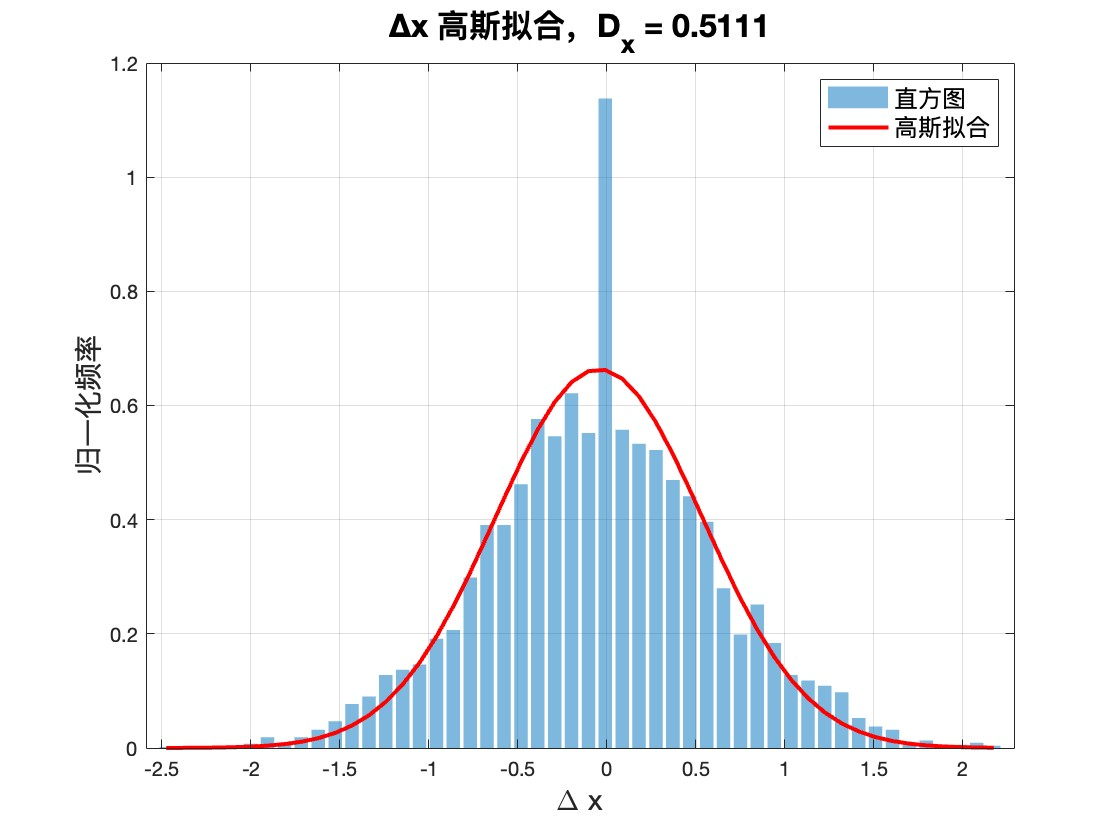
\includegraphics[width=\textwidth]{Fig_5.jpg}
                    \caption{$x$ 方向的拟合}
                    \label{fig:GaussX}
                \end{minipage}
                \begin{minipage}{0.47\textwidth}
                    \centering
                    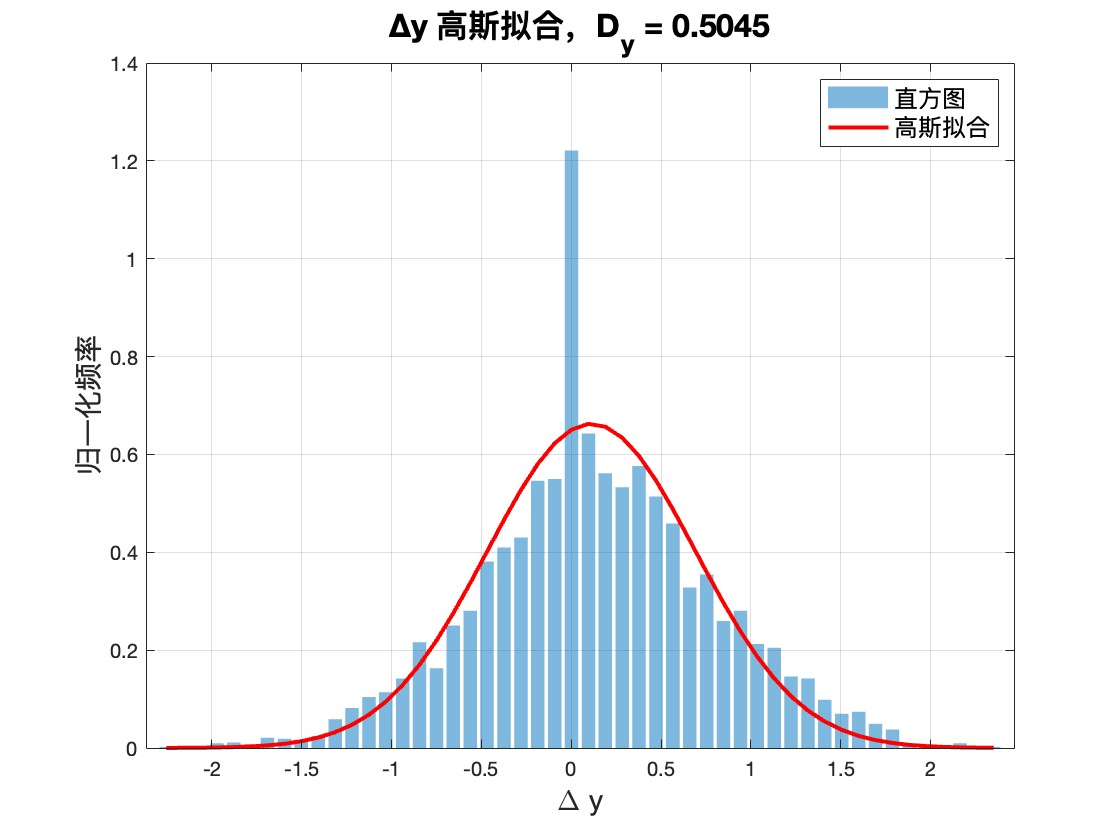
\includegraphics[width=\textwidth]{Fig_6.jpg}
                    \caption{$y$ 方向的拟合}
                    \label{fig:GaussY}
                \end{minipage}
            \end{figure}

            \item \textbf{误差分析：}
            \begin{enumerate}[left = 0pt]
                \item 布朗运动有较大随机性，因此在观测数据不足时，难以精确拟合计算，具有较大偶然性。
                \item 实验采用制作流道的方式观察荧光小球的运动，在实际操作中，制作装片、安放装片、调整载物台位置时均有可能使装片中的液体流动。因此微粒可能在布朗运动的基础上还叠加定向运动，这使得计算得到的扩散系数偏大，间接导致了 $k$ 偏大，$N_\text{A}$ 偏小。
                \item 实验才有小球本身作为比例尺，默认小球直径为 \qty{1}{\micro \m}，并据此在图像中确认像素的大小。然而图像中的小球未必时刻都处于焦平面上，这使得确定小球的边界变得困难。同时为了使观察清晰，实验中不得已调整观察的焦平面，这也会使图像的比例变化，造成误差。
            \end{enumerate}
        \end{enumerate}
    
    \item 思考题
    \begin{enumerate}[label=\arabic*.,left = 0pt]
        \item 一维布朗运动的模拟：采用如下代码在 Matlab 中模拟一维随机运动。
        \begin{lstlisting}
numSteps = 1000;      
numTrials = 1000;     
stepSize = 1;         

all_positions = zeros(numTrials, numSteps);

for i = 1:numTrials
    steps = randi([0,1], 1, numSteps) * 2 - 1;  
    positions = cumsum(steps * stepSize);      
    all_positions(i, :) = positions;
end
            
msd = mean(all_positions.^2, 1);              
theory = stepSize^2 * (1:numSteps);
            
figure;
plot(1:numSteps, msd, 'b', 'LineWidth', 2); hold on;
plot(1:numSteps, theory, 'r--', 'LineWidth', 2);
xlabel('步数 n');
ylabel('均方位移 \langle x^2 \rangle');
legend('模拟值', '理论值 n\delta^2', 'Location', 'northwest');
title('一维随机运动的均方位移');
grid on;
        \end{lstlisting}
        根据理论预测，$\langle x^2 \rangle = n\delta^2 = n$。实际 Matlab 所绘制的图像如图~\ref{fig:Simulation}，可见模拟与理论预测由较好符合。
        \begin{figure}[h]
            \centering
            
\includegraphics[width=0.75\linewidth]{Fig_1.jpg}
            \caption{一维布朗运动模拟}
            \label{fig:Simulation}
        \end{figure}

        \item 定向运动与随机扩散：定向运动的均方位移与时间的平方成正比，而随机扩散运动的均方位移与时间成正比。图~\ref{fig:comparison}是两者运动模式的对比。可以发现，短程位移随机扩散快于定向运动，而长程位移定向运动快于随机扩散。
        \begin{figure}[h]
            \centering
            
\includegraphics[width=0.75\linewidth]{Fig_2.jpg}
            \caption{定向运动与随机扩散对比}
            \label{fig:comparison}
        \end{figure}
        
    \end{enumerate}

\end{enumerate}
\end{document}